\chapter{Cloud Computing \& Outsourcing}

\section{Sie verstehen die grundlegende Theorie des Cloud Computing (IaaS, PaaS und SaaS).}

Die Definition von Cloud Computing lautet wie folgt und ist prüfungsrelevant:
\quote{Cloud Computing ist ein Modell respektive beschreibt den Ansatz, um IT-Applikationen (Services) aber Plattformen und IT-Infrastrukturen nach Bedarf dynamisch erweiterbar über ein Netzwerk zur Verfügung zu stellen.}

Cloud Computing ist im Kern eine Outsourcing-Technik, bei der interne IT-Aufgaben an ein externes Unternehmen ausgelagert werden. Die Dienstleistung befindet sich in einer ''Wolke'' verhüllt und wird über eine definierte Schnittstelle bezogen.

Eine Cloud-Infrastruktur sollte folgende Eigenschaften aufweisen:
\begin{description}
	\item[On Demand Self Service:] Der Nutzer kann sich eine Leistung aus der Cloud selbst zuweisen und diese muss auch zur Verfügung stehen.
	\item[Scalability:] Funktionen können schnell und dynamisch bereitgestellt werden. Dem Nutzer sollte eine ''unlimitierte'' Kapazität zur Verfügung stehen.
	\item[Broad Network Acces:] Die Services stehen über ein Netzwerk zur Verfügung und können auf unterschiedlichen Plattformen genutzt werden.
	\item[Resource Pooling:] Computer Ressourcen (Speicher, Netzwerk usw.) werden gebündelt und virtualisiert. Sie können dadurch dynamisch verteilt werden und der Nutzer weiss nicht von welchen Server der Service kommt.
	\item[Measured Service:] Die Cloudsysteme können ständig überwacht und die Qualität sichergestellt werden. Dies ermöglicht Transparenz für den Anbieter als auch den Nutzer.
\end{description}

Abbildung \ref{fig:cloud-erbringung} zeigt die drei Ebenen der Cloud-Service Erbringung. Diese werden in den folgenden Abschnitten detailliert beschrieben. 

\begin{figure}
\centering
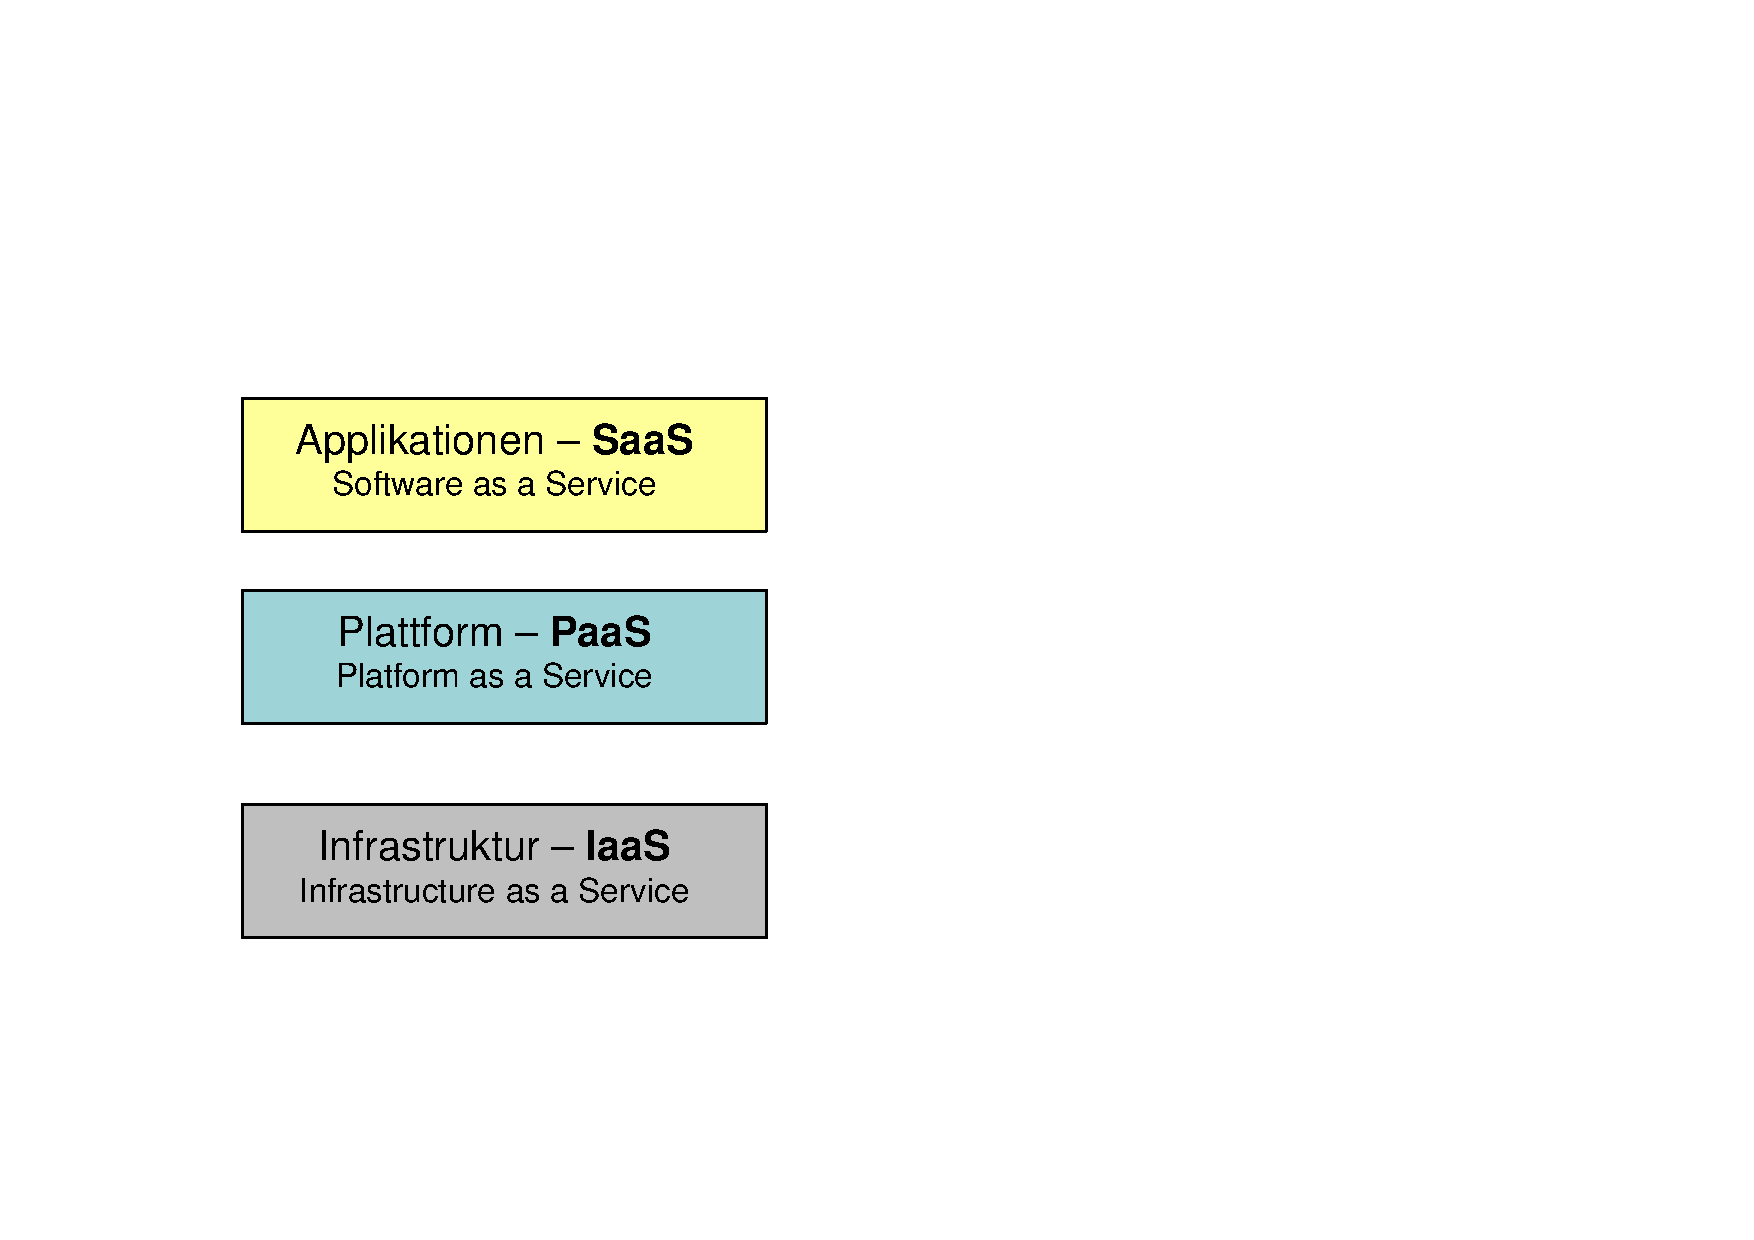
\includegraphics[width=0.5\linewidth]{fig/cloud-erbringung}
\caption{}
\label{fig:cloud-erbringung}
\end{figure}

\subsection{SaaS - Software as a Service}

Die oberste Ebene umfasst Anwendungen. Anwendungen werden als standardisierte Services bereitgestellt und lassen sich nur eingeschränkt anpassen. Diese Ebene richtet sich an Privatkunden und Business Analysten. Bekannte Beispiele sind Dropbox, Office 365 oder ERP-Systeme.

\subsection{PaaS - Platform as a Service}

Eine Ebene darunter liegen die Services für Entwicklungs-Plattformen. Mit diesen Services lassen sich Anwendungen entwickeln und integrieren. Diese Ebene richtet sich an Architekten und Anwendungsentwickler. Beispiele für Services sind Datenbanken oder Applikationsserver.

\subsection{IaaS - Infrastructure as a Service}

Auf der untersten Ebene ist die Infrastruktur angesiedelt. Es werden Rechen-, Speicher- oder Netzwerkleistungen über virtualisierte Server bereitgestellt. Diese Ebene richtet sich an den IT-Betrieb.

\section{Sie kennen die wichtigsten Prinzipien für eine Cloud-Architektur und können diese bewerten und in der IT-Landschaft einordnen.}

Eine Cloud kann auf verschiedene Arten organisiert werden. Es werden folgende Organisationsformen unterschieden:
\begin{description}
	\item[Public Cloud:] Die Cloud-Umgebung befindet sich beim IT-Dienstleister und wird auch von diesem betrieben. Auf eine Public Cloud wird über das Internet zugegriffen und diese wird meist auf einer ''pay per use''-Basis abgerechnet.
	\item[Private Cloud:] Die Cloud-Umgebung befindet sich beim Kunden und wird auch von diesem betrieben. Auf eine Private Cloud kann über das firmeneigene Intranet zugegriffen werden. Da der Kunde die Kontrolle über die Cloud hat, kann er individuelle Anpassungen vornehmen.
	\item[Hybrid Cloud:] Eine Hybrid Cloud ist eine Mischform zwischen Private und Public Cloud und ist in der Praxis am häufigsten anzutreffen.
	\item[Community Cloud:] Die Community Cloud wird von einer kleinen Gruppe von Organisationen betrieben. Ein Beispiel wäre eine Cloud welche alle Hochschulen nutzen.
\end{description}

Die folgende Aufzählung zeigen die Vor- und Nachteile einer Cloud:
\begin{itemize}
	\item Vorteile:
	\begin{itemize}
		\item Nutzer müssen Server- und Software nicht selber anschaffen
		\item Die Kosten sind variabel und können nach Bedarf (Nutzung) angepasst werden.
		\item Die Kosten sind tendenziell tiefer wegen der Ausnutzung von Grössenvorteilen.
		\item Bedarf an technischem Know How sinkt, Fokus auf das Kerngeschäft
		\item Firmen, welche Cloud-Services anbieten, bieten eine katastrophensichere Aufbewahrung der Daten.
		\item Der Zugriff auf die Daten ist von überall her möglich.
		\item Kosten- und Personalintensive Implementierungen können vermieden werden
		\item Gute Skalierbarkeit: Erweiterung oder neue Dienstleistungen können selbstständig bestellt werden und sind sofort verfügbar
	\end{itemize}
	\item Nachteile:
	\begin{itemize}
		\item Datenschutz und Sicherheit der Daten, diese sind irgendwo gespeichert,
		\item Absicherung des Zugriffs auf die Daten (Verschlüsselung)
		\item Zuverlässigkeit des Providers, Qualität \& Stabilität des Services
		\item Starke Bindung an den Provider (Vendor Locking)
		\item Katastrophenschutz, wie ist der Service gewährleistet im Falle einer Katastrophe
	\end{itemize}
\end{itemize}

\section{Sie verstehen was Outsourcing ist und kennen die möglichen Ausprägungen.}

Outsourcing wird aus den drei Begriffen Outside + Resource + Using zusammengesetzt. Mit Outsourcing ist die signifikante Beteiligung von externen Firmen bei der Erbringung von IT Services mittels Mitarbeiter und IT Komponenten innerhalb Firmen. Outsourcing beinhaltet die Frage, ob bestimmte Aktivitäten intern oder von einem externen Anbieter erbracht werden sollen (make or buy).

Outsourcing wird vielfach als Antwort auf eine Marktveränderung eingeführt. Dabei sind drei Hauptgründe die Motivation dafür:
\begin{enumerate}
	\item Kosten und Flexibilität
	\item Finanzielle Überlegenheit
	\item Technische Überlegenheit
\end{enumerate}

Die Gründe für Outsourcing sind vielfältig. Nachfolgend sind einige Gründe aus verschiedenen Perspektiven aufgelistet.
\begin{itemize}
	\item Management
	\begin{itemize}
		\item Reduuktion der IT-Kosten
		\item Erhöhung der Transparenz (Business misstraut der internen IT bezüglich Effizienz)
		\item Konzentration auf Kernkompetenzen (Womit man Geld verdient)
		\item Qualität und Effizienz der IT steigern
	\end{itemize}
	\item Kosten
	\begin{itemize}
		\item Kostenrduktion durch Grössenvorteil (z.B. Swisscom hat mehr IT-Kunden im Tessin als Credit Suisse)
		\item Umwandlung Fixkosten in variable Kosten (Bessere Planbarkeit und Transparenz)
	\end{itemize}
	\item Technologie
	\begin{itemize}
		\item Zugang zu speziellem Know-How (Stärkere Innovationskraft, moderne Technologien)
		\item Verlagerung von Risiken (neue Technologie und Komplexität) zum Outsourcing-Anbieter
	\end{itemize}
	\item Personal
	\begin{itemize}
		\item Keine Personalknappheit/-überschuss zu Spitzenzeiten (Skalierbarkeit)
		\item Verringerung des IT-Personals (Keine Abhängigkeit von Mitarbeitern mit speziellem Know-How)
	\end{itemize}
	\item Finanzen
	\begin{itemize}
		\item Vermeidung von hohen Investitionen in neue Technologien
		\item Gebundenes Kapital (z.B. Hardware) kann verkauft werden und dadurch z.B. Jahresabschluss beeinflusst werden.
	\end{itemize}
\end{itemize}

\section{Sie kennen die Beweggründe sowie Risiken und Strategien des Outsourcing}

Abbildung \ref{fig:outsourcing-strategie} zeigt die verschiedenen Outsourcing Strategien.
\begin{figure}
\centering
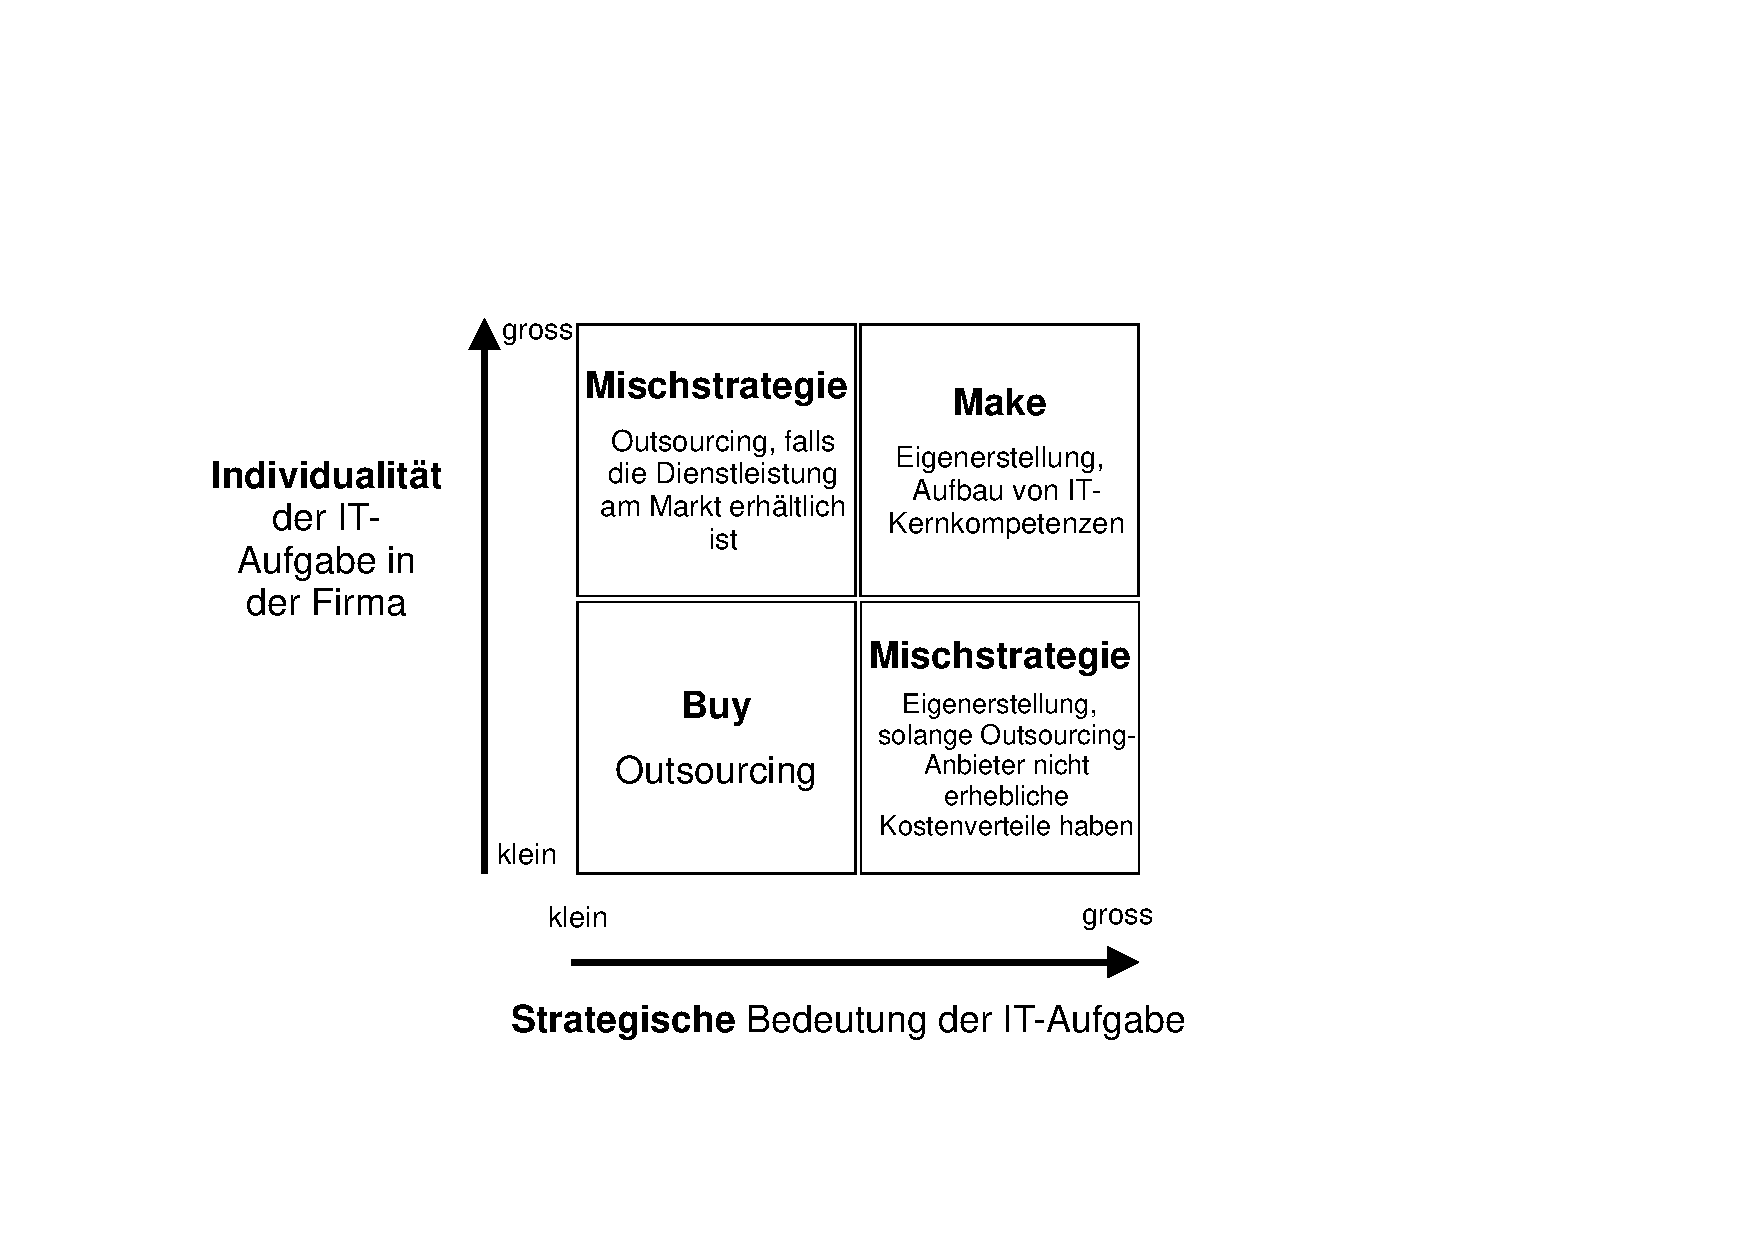
\includegraphics[width=0.7\linewidth]{fig/outsourcing-strategie}
\caption{Outsourcing Strategien}
\label{fig:outsourcing-strategie}
\end{figure}
Das Outsourcing bringt auch zahlreiche Risiken mit sich. Die Hauptrisiken sind:
\begin{itemize}
	\item hohe Abhängigkeit
	\item Verlust der Sicherheit
	\item Know-How Verlust
	\item Personalpolitik
\end{itemize}
Aus der Sicht des Management ist die grosse Abhängigkeit vom Outsourcing-Anbieter ein Problem. Durch die langfristige Bindung an einen Anbieter (üblich 3-6 Jahre) kann ein Umstieg evtl. nicht mehr rückgängig gemacht werden. Auch die räumliche Distanz bringt oft Probleme mit sich. 
Auch steigende Kosten können zu einem Risiko werden. Kosten entstehen bei der Evaluation, der Umstellung und auch durch erhöhten Koordinationsaufwand während des Betriebs. Hat der Outsourcing-Anbieter wenig Konkurrenz kann er die Preise festlegen (Vendorlocking) und es entstehen intransparente Preise.
Bei der Technologie kann IT-spezifische Kompetenzen verloren gehen und auch durch die Standardisierung wird die Serviceerbringung nicht mehr flexibel.
Bei der Auslagerung von Daten kann man mit dem Gesetz in Konflikt kommen (Datenschutz) oder firmenrelevante Daten komplett verlieren.
Beim Personal können Schlüsselpersonen und Know-How verloren gehen. Auch die Unternehmenskultur kann unter einem Outsourcing leiden.
Die oben genannten Risiken können teilweise so stark werden, dass ein Re-/Insourcing durchgeführt werden muss. Dabei wird die ausgelagerten Services wieder in die eigene IT eingegliedert, was mit sehr hohem Aufwand verbunden sein kann.

